\documentclass[10pt,aspectratio=169,xcolor={table}]{beamer}

\usetheme{Madrid}
\setbeamertemplate{navigation symbols}{}
\setbeamertemplate{blocks}[rounded][shadow=false]

\usepackage{tikz}
\usepackage{pgfplots}
\pgfplotsset{compat=1.15}
\usepackage{listings}
\usepackage{booktabs}
\usepackage{amsmath}

\definecolor{kw}{RGB}{0,60,160}
\definecolor{cm}{RGB}{100,100,100}
\definecolor{st}{RGB}{170,60,0}

\lstdefinestyle{py}{
  language=Python,
  basicstyle=\ttfamily\scriptsize,
  keywordstyle=\color{kw}\bfseries,
  commentstyle=\color{cm}\itshape,
  stringstyle=\color{st},
  showstringspaces=false,
  frame=single,
  rulecolor=\color{black!30},
  breaklines=true,
  morekeywords={Bool,Int,Distinct,Or,Not,Solver,sat,unsat,model}
}
\lstdefinestyle{sh}{
  language=bash,
  basicstyle=\ttfamily\scriptsize,
  keywordstyle=\color{kw}\bfseries,
  commentstyle=\color{cm}\itshape,
  showstringspaces=false,
  frame=single,
  rulecolor=\color{black!30},
  breaklines=true
}

\title[Pigeonhole with Z3]{The Pigeonhole Problem\\[1mm]\large A Performance Study with the Z3 SMT Solver\\[2mm]{\normalsize Self-Study Presentation}}
\author[I.~Sharma \textbar\ 25B2270]{Ishan Sharma\\[1mm]{\small Roll No.\ 25B2270}}
\institute[IIT Bombay]{Indian Institute of Technology Bombay}
\date{November 2026}

\begin{document}

% ---------------- title ----------------
\begin{frame}
  \titlepage
\end{frame}

\begin{frame}{Contents}
  \tableofcontents
\end{frame}

% =====================================================
\section{Background: From DPLL to CDCL}
% =====================================================

\begin{frame}[fragile]{DPLL (1962): the Classic Backtracking Search}
  \begin{itemize}\itemsep2pt
    \item Davis--Putnam--Logemann--Loveland: decide SAT of a CNF
          formula by \textbf{backtracking search over truth
          assignments}.
    \item Two cheap inference rules prune the tree:
          \textbf{unit propagation} (a literal alone in a clause
          is forced) and \textbf{pure-literal elimination}.
    \item On conflict, backtrack and try the other value ---
          worst case $2^{\#vars}$ branches.
    \item Complete and still the \emph{skeleton} of every modern
          SAT solver --- what changed is how cleverly the tree is
          pruned.
  \end{itemize}
\begin{lstlisting}[basicstyle=\ttfamily\scriptsize,frame=single,rulecolor=\color{black!30}]
def DPLL(clauses, assignment):
    if all clauses are satisfied:   return SAT
    if some clause is empty:        return UNSAT    # conflict -> backtrack
    unit_propagate(clauses)         # literal alone in a clause -> forced
    remove_pure_literals(clauses)   # variable with one sign -> assign it
    x = pick an undecided variable
    return DPLL(clauses with x = True) or DPLL(clauses with x = False)
\end{lstlisting}
\end{frame}

\begin{frame}{CDCL (1996--): DPLL that Remembers Its Mistakes}
  \begin{itemize}\itemsep4pt
    \item \textbf{Conflict-Driven Clause Learning}: when unit
          propagation hits a contradiction, \emph{analyse the
          conflict} and derive a \textbf{learned clause} that
          explains it --- that failed branch can never be
          re-explored again.
    \item \textbf{Non-chronological backtracking}: jump directly
          back to the decision that caused the conflict.
    \item Engineering that made it fly: \textbf{watched literals}
          (constant-time propagation bookkeeping),
          \textbf{VSIDS} (branch on recently active variables),
          \textbf{periodic restarts}.
    \item Lineage: GRASP/Chaff $\to$ MiniSat (2003) $\to$
          CaDiCaL/Kissat --- and \textbf{Z3's SAT core}.
  \end{itemize}
  \begin{block}{The one-sentence difference}
    DPLL forgets every failed branch; CDCL compresses each failure
    into a clause so the same mistake is never made twice.
  \end{block}
\end{frame}

\begin{frame}{Non-Chronological Backtracking: One Jump Kills a Subtree}
  \centering
  {\small $C_1{=}(p \lor \lnot r)$,\; $C_2{=}(r \lor u)$,\;
          $C_3{=}(r \lor \lnot u)$,\; $C_4{=}(\lnot p \lor q)$,\;
          $C_5{=}(\lnot p \lor \lnot q)$ \quad --- \quad UNSAT}

  \medskip
  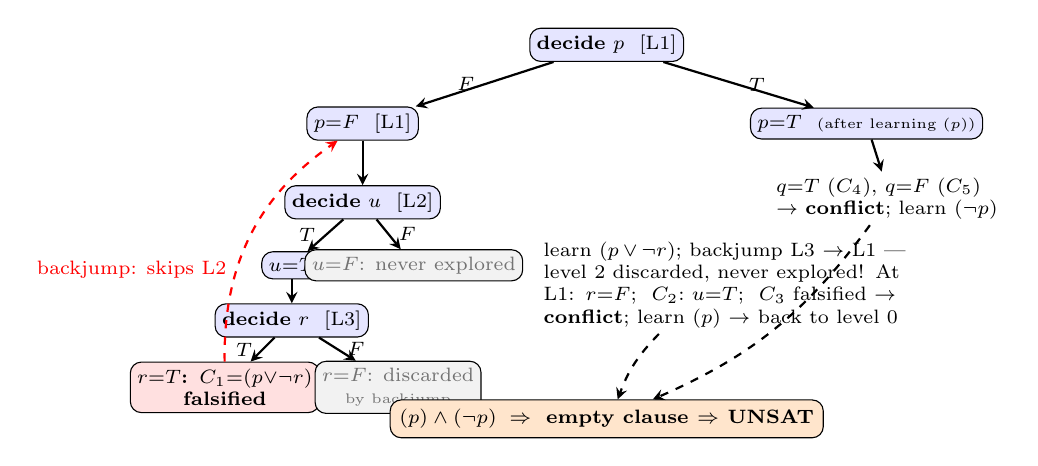
\begin{tikzpicture}[>=stealth,
    dec/.style={draw,rounded corners,fill=blue!10,align=center,font=\scriptsize,inner sep=2.5pt},
    dead/.style={draw,rounded corners,fill=black!5,align=center,font=\scriptsize,inner sep=2.5pt,text=black!55},
    conf/.style={draw,rounded corners,fill=red!12,align=center,font=\scriptsize\bfseries,inner sep=2.5pt},
    note/.style={align=left,font=\scriptsize,inner sep=2pt}]
    \node[dec] (A) at (5.4,5.0) {\textbf{decide} $p$ \ [L1]};
    \node[dec] (B) at (2.3,4.0) {$p{=}F$ \ [L1]};
    \node[dec] (C) at (8.7,4.0) {$p{=}T$ \ {\tiny (after learning $(p)$)}};
    \node[dec] (D) at (2.3,3.0) {\textbf{decide} $u$ \ [L2]};
    \node[dec] (E) at (1.4,2.2) {$u{=}T$};
    \node[dead] (F) at (2.95,2.2) {$u{=}F$: never explored};
    \node[dec] (G) at (1.4,1.5) {\textbf{decide} $r$ \ [L3]};
    \node[conf] (H) at (0.55,0.65) {$r{=}T$: $C_1{=}(p{\lor}\lnot r)$\\ falsified};
    \node[dead] (I) at (2.75,0.65) {$r{=}F$: discarded\\ {\tiny by backjump}};
    \node[note,text width=4.6cm] (K) at (6.9,1.95) {learn $(p \lor \lnot r)$;
      \alert{backjump L3 $\to$ L1} --- level 2 discarded, never explored!
      At L1: $r{=}F$; \ $C_2{:}\ u{=}T$; \ $C_3$ falsified $\to$ \textbf{conflict};
      learn $(p)$ $\to$ back to level 0};
    \node[note,text width=2.9cm] (L) at (9.0,3.05) {$q{=}T$ $(C_4)$, $q{=}F$ $(C_5)$
      $\to$ \textbf{conflict}; learn $(\lnot p)$};
    \node[draw,rounded corners,fill=orange!20,font=\scriptsize\bfseries,align=center] (M) at (5.4,0.25)
      {$(p) \wedge (\lnot p) \;\Rightarrow\;$ empty clause $\Rightarrow$ \textbf{UNSAT}};
    \draw[->,thick] (A) -- node[left,font=\scriptsize] {$F$} (B);
    \draw[->,thick] (A) -- node[right,font=\scriptsize] {$T$} (C);
    \draw[->,thick] (B) -- (D);
    \draw[->,thick] (D) -- node[left,font=\scriptsize] {$T$} (E);
    \draw[->,thick] (D) -- node[right,font=\scriptsize] {$F$} (F);
    \draw[->,thick] (E) -- (G);
    \draw[->,thick] (G) -- node[left,font=\scriptsize] {$T$} (H);
    \draw[->,thick] (G) -- node[right,font=\scriptsize] {$F$} (I);
    \draw[->,thick,dashed,red] (H) to[bend left=28]
      node[pos=0.35,left,font=\scriptsize,text=red] {backjump: skips L2} (B);
    \draw[->,thick] (C) -- (L);
    \draw[->,thick,dashed] (K) to[bend right=12] (M);
    \draw[->,thick,dashed] (L) to[bend left=15] (M);
  \end{tikzpicture}

  \medskip
  {\scriptsize A chronological (DPLL) solver would now grind through the
   $u{=}F$ subtree. CDCL's learned clause $(p \lor \lnot r)$ proves $u$
   irrelevant to the conflict --- the entire level-2 subtree is skipped
   in one jump. The run still ends UNSAT.}
\end{frame}

\begin{frame}{Resolution: Why Some Formulas Stay Hard Forever}
  \begin{columns}[T]
    \begin{column}{0.52\textwidth}
      \begin{itemize}\itemsep3pt
        \item \textbf{Resolution rule} --- combine two clauses on a
          complementary literal:
          \[
            \frac{A \lor x \qquad B \lor \lnot x}{A \lor B}
          \]
        \item Refutationally complete: a formula is UNSAT
          $\iff$ repeated resolution derives the \emph{empty
          clause}.
        \item CDCL's learned clauses \emph{are} resolution
          derivations: CDCL (with restarts) polynomially simulates
          resolution, and vice versa (Pipatsrisawat \& Darwiche,
          2009).
      \end{itemize}
    \end{column}
    \begin{column}{0.44\textwidth}
      \begin{itemize}\itemsep3pt
        \item \textbf{Haken (1985)}: the pigeonhole principle has
          \emph{no polynomial-size resolution proof} ---
          exponentially many clauses are unavoidable.
        \item $\Rightarrow$ every CDCL prover must grind out
          exponentially many learned clauses on it.
        \item \alert{This is exactly the effect we will measure
          with Z3.}
      \end{itemize}
    \end{column}
  \end{columns}
\end{frame}

% =====================================================
\section{Z3: SMT on Top of CDCL}
% =====================================================

\begin{frame}{Z3 and the CDCL(T) Architecture}
  \begin{itemize}\itemsep3pt
    \item \textbf{Z3} (Microsoft Research; de Moura \& Bj{\o}rner,
          TACAS 2008): an \textbf{SMT} solver --- satisfiability
          \emph{modulo theories}: CDCL over a propositional
          abstraction + dedicated theory solvers (integer
          arithmetic, arrays, bit-vectors, distinctness, \dots).
          Python API: the \texttt{z3-solver} package.
    \item Architecture, per \emph{Programming Z3} \S6.1.1: the SAT
          solver enumerates truth assignments to atoms (a
          \emph{propositional abstraction} of the formula), and
          \emph{theory solvers} check each assignment modulo the
          theories.
    \item Classically called \textbf{DPLL(T)}; Z3 says
          \textbf{CDCL(T)} because its SAT engines use
          conflict-driven clause learning --- ``which goes beyond
          the algorithm associated with DPLL''.
    \item Learned clauses block future case splits from
          re-exploring failed branches; efficient solvers add
          \emph{theory propagation} between theories and the SAT
          core.
  \end{itemize}
\end{frame}

\begin{frame}[fragile]{Reading z3py --- the API Used Throughout (\emph{Programming Z3} \S2)}
\begin{lstlisting}[style=py]
from z3 import *
Tie, Shirt = Bools('Tie Shirt')          # declare Boolean variables
s = Solver()
s.add(Or(Tie, Shirt),                    # constraints = assertions
      Or(Not(Tie), Shirt),
      Or(Not(Tie), Not(Shirt)))
print(s.check())                         # sat / unsat / unknown
print(s.model())                         # e.g. [Tie = False, Shirt = True]
\end{lstlisting}
  \begin{itemize}\itemsep1pt
    \item \texttt{Bools / Bool / Ints / Int} --- declare variables;
          \texttt{Or / And / Not / Implies} --- connectives;
          \texttt{==} between Booleans means bi-implication.
    \item \texttt{Solver()} accumulates constraints via
          \texttt{s.add(...)}; \texttt{s.check()} decides;
          \texttt{s.model()} extracts a satisfying assignment.
    \item Theory constraints read like ordinary Python over
          \texttt{Int}s: \texttt{0 <= h[i]}, \texttt{h[i] < n},
          \texttt{Distinct(h)} --- exactly Encoding II later.
    \item \texttt{s.set("timeout", ms)} --- per-solver cap (used by
          the benchmark).
    \item Example verbatim from \emph{Programming Z3} \S2 --- the
          syntax the online CDCL(T) code on the next slides assumes.
  \end{itemize}
\end{frame}

\begin{frame}[fragile]{CDCL(T) in Code (1/2) --- Abstraction Helpers (Fig.~13)}
\begin{lstlisting}[style=py,basicstyle=\ttfamily\tiny]
index = 0
def abstract_atom(abs, atom):
    # abs = dictionary: theory atom (e.g. x >= 0)  ->  Bool variable
    if atom in abs:
        return abs[atom]      # seen this atom before: reuse its Bool
    p = Bool("p%d" % index)   # else invent a fresh variable p0, p1, ...
    index += 1
    abs[atom] = p             # remember the atom <-> Bool correspondence
    return p

def abstract_lit(abs, lit):
    # a literal is an atom or its negation; abstract it consistently
    if is_not(lit):
        return Not(abstract_atom(abs, lit.arg(0)))
    return abstract_atom(abs, lit)

def abstract_clause(abs, clause):
    # clause = OR of theory literals -> OR of Bool literals
    return Or([abstract_lit(abs, lit) for lit in clause])

def abstract_clauses(abs, clauses):
    # whole formula: list of clauses -> pure Boolean clause list
    return [abstract_clause(abs, clause) for clause in clauses]

def mk_lit(m, p):
    # read the value of Bool p out of a model m:  True -> p, False -> Not p
    if is_true(m.eval(p)):
        return p
    else:
        return Not(p)
\end{lstlisting}
  {\scriptsize Code verbatim from \emph{Programming Z3} (Fig.~13); comments
   added here. It maps every theory atom to a fresh Boolean variable ---
   building the propositional abstraction the SAT core works on.}
\end{frame}

\begin{frame}[fragile]{CDCL(T) in Code (2/2) --- the Solver Loop (Fig.~12)}
\begin{lstlisting}[style=py,basicstyle=\ttfamily\tiny]
def simple_cdclT(clauses):
    # two solvers:  prop   = the SAT core (sees only Booleans)
    #               theory = checks the real atoms (arithmetic, ...)
    prop   = Solver()
    theory = Solver()
    abs = {}                                    # atom -> Bool variable
    # SAT core receives the abstracted, pure-Boolean problem
    prop.add(abstract_clauses(abs, clauses))
    # theory solver receives the link: each p is equivalent to its atom
    theory.add([p == abs[p] for p in abs])
    while True:
        is_sat = prop.check()          # 1. SAT core PROPOSES an assignment
        if sat == is_sat:
            m = prop.model()
            # translate the Boolean assignment back into theory literals
            lits = [mk_lit(m, abs[p]) for p in abs]
            # 2. ask the theory solver: is this assignment really consistent?
            if unsat == theory.check(lits):
                # 3. NO: unsat_core() = the conflicting subset of lits
                #    block exactly that combination -- a LEARNED clause:
                prop.add(Not(And(theory.unsat_core())))
                #    ^ the "learn -> backjump" step from the tree slide
            else:
                # 4. consistent modulo theories -> genuine solution
                print(theory.model())
                return
        else:
            print(is_sat)              # SAT core proved abstraction UNSAT
            return
\end{lstlisting}
  {\scriptsize Code verbatim from \emph{Programming Z3} (\S6.1.1, Fig.~12);
   comments added. Steps 1--4 = propose, check, \alert{learn}, accept. The
   pigeonhole analysis counts how many learned clauses (step 3) the
   principle forces.}
\end{frame}

\begin{frame}[fragile]{Working Environment}
\begin{lstlisting}[style=sh]
$ python3 -m venv venv && source venv/bin/activate
(venv)$ pip install z3-solver        # z3-solver 5.4.1, Python 3.14
(venv)$ python pigeonhole.py         # encodes, solves, times it
\end{lstlisting}
  \begin{itemize}\itemsep2pt
    \item Isolated venv, pinned solver version --- results are
          reproducible with the three commands above.
    \item Z3 itself is open source:
          \texttt{github.com/Z3Prover/z3}.
  \end{itemize}
\end{frame}

% =====================================================
\section{The Pigeonhole Problem}
% =====================================================

\begin{frame}{The Problem}
  \begin{columns}[T]
    \begin{column}{0.52\textwidth}
      \begin{itemize}\itemsep3pt
        \item \textbf{Formulation}: place $m$ pigeons into $n$
          holes such that
          \begin{itemize}
            \item every pigeon occupies at least one hole:
                  $\bigvee_j x_{ij}$,
            \item no hole holds two pigeons:
                  $\lnot x_{ij} \lor \lnot x_{kj}$ for $i<k$.
          \end{itemize}
        \item \textbf{Theorem}: satisfiable $\iff m \le n$.
        \item Trivial for humans, yet refuting the $m>n$ case is
          provably hard for computers --- a classic
          \emph{proof-complexity} benchmark.
        \item This asymmetry (easy SAT, hard UNSAT) is exactly
          what the study measures.
      \end{itemize}
    \end{column}
    \begin{column}{0.44\textwidth}
      \centering
      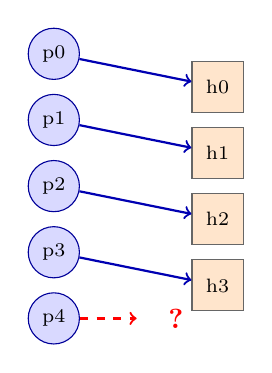
\begin{tikzpicture}[scale=0.8,
        pigeon/.style={circle,draw=blue!60!black,fill=blue!15,minimum size=6.5mm,inner sep=0},
        hole/.style={rectangle,draw=black!60,fill=orange!20,minimum size=6.5mm,inner sep=0}]
        \foreach \i in {0,...,4}
          \node[pigeon] (q\i) at (0,-1.05*\i) {\scriptsize p\i};
        \foreach \i in {0,...,3}
          \node[hole] (g\i) at (2.6,-1.05*\i-0.525) {\scriptsize h\i};
        \foreach \i in {0,...,3}
          \draw[->,thick,blue!70!black] (q\i) -- (g\i);
        \draw[->,thick,dashed,red] (q4.east) -- ++(0.9,0);
        \node[red] at (q4.east) [right=1.0cm] {\textbf{?}};
      \end{tikzpicture}

      \medskip
      {\scriptsize $m=5$, $n=4$: some hole must hold
       $\ge 2$ pigeons $\Rightarrow$ UNSAT}
    \end{column}
  \end{columns}
\end{frame}

\begin{frame}[fragile]{Encoding I --- Boolean CNF (SAT style)}
  \begin{itemize}\itemsep1pt
    \item One variable $x[i][j]$ = ``pigeon $i$ sits in hole $j$''.
    \item Size: $m\cdot n$ variables, $m + n\binom{m}{2}$ clauses
          (e.g.\ $12/11$: 132 vars, 738 clauses).
    \item The pairwise CNF form is the standard encoding in the
          SAT literature --- the same form as the crafted
          \texttt{php\_*.cnf} pigeonhole instances used by SAT
          benchmark suites.
  \end{itemize}
\begin{lstlisting}[style=py]
x = [[Bool(f"p{i}_{j}") for j in range(n)] for i in range(m)]

for i in range(m):                     # pigeon i needs a hole
    s.add(Or(x[i]))

for j in range(n):                     # hole j holds <= 1 pigeon
    for i, k in itertools.combinations(range(m), 2):
        s.add(Or(Not(x[i][j]), Not(x[k][j])))
\end{lstlisting}
\end{frame}

\begin{frame}[fragile]{Encoding II --- Integer + Distinct (SMT style)}
\begin{lstlisting}[style=py]
h = [Int(f"h{i}") for i in range(m)]   # hole index per pigeon
for i in range(m):
    s.add(0 <= h[i], h[i] < n)         # domain [0, n)
s.add(Distinct(h))                     # no two pigeons share a hole
\end{lstlisting}
  \begin{itemize}\itemsep2pt
    \item Compact: only $m$ integer variables, $2m+1$ constraints.
    \item But Z3 must reason with \emph{arithmetic};
          \texttt{Distinct} internally expands to $\binom{m}{2}$
          disequalities.
    \item Hypothesis going in: compact \alert{statement} $\ne$
          efficient \alert{proof} --- tested in the experiments.
  \end{itemize}
\end{frame}

\begin{frame}[fragile]{Source and Reproducibility}
  \begin{itemize}\itemsep2pt
    \item \textbf{This study's source} (script + these slides):
          \\ \texttt{github.com/IshanIITB/pigeonhole-z3}
    \item \textbf{Solver}: \texttt{github.com/Z3Prover/z3} ---
          full source of Z3, including its CDCL SAT core.
    \item Reference online projects (verified):
          \texttt{github.com/martadavma/PigeonholePrinciple}
          (bare Z3 example --- \emph{no} timeout),
          \texttt{github.com/bushesarebetter/sat-solver}
          (DPLL benchmarked on \texttt{php\_*.cnf} with a 10\,s
          per-instance cap).
    \item Full listing of \texttt{pigeonhole.py} in the appendix;
          benchmark protocol and raw output follow the results.
  \end{itemize}
  \begin{block}{Benchmark protocol}
    Nine $(m,n)$ pairs: SAT cases ($m\le n$), tight UNSAT
    ($m=n+1$), loose UNSAT ($m\gg n$); expected answer known
    a priori for cross-checking. Metric: wall-clock time of
    \texttt{s.check()} via \texttt{time.perf\_counter()}, both
    encodings on every instance.
  \end{block}
\end{frame}

\begin{frame}[fragile]{The 20\,s Per-Instance Timeout}
\begin{lstlisting}[style=py]
TIMEOUT_MS = 20_000
s.set("timeout", TIMEOUT_MS)     # inside every encoder, caps each check()
\end{lstlisting}
  \begin{itemize}\itemsep2pt
    \item \alert{The cap is a benchmarking choice, not part of the
          problem}: quick online Z3 examples run bare
          \texttt{check()} with no limit, but benchmark harnesses
          do set one --- the DPLL project above caps at 10\,s;
          SAT Competition harnesses likewise.
    \item Without a cap, the hardest UNSAT instances simply run
          unbounded and the benchmark never terminates.
    \item A timed-out instance yields \texttt{unknown} ---
          \emph{undecided}, not unsat; the expected answer comes
          from the theorem, not the solver.
  \end{itemize}
\end{frame}

% =====================================================
\section{Results}
% =====================================================

\begin{frame}{Observation 1 --- the SAT Side Is Trivial ($m=n=8$, $\sim$1\,ms)}
  \centering
  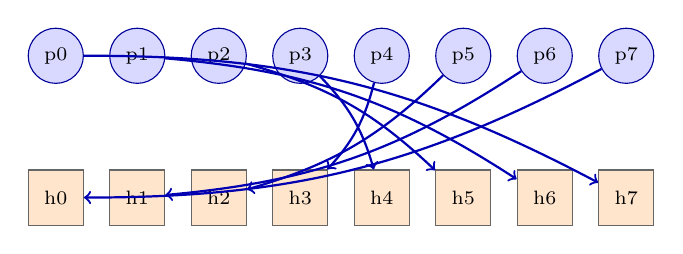
\begin{tikzpicture}[scale=0.9,
    pigeon/.style={circle,draw=blue!60!black,fill=blue!15,minimum size=7mm,inner sep=0},
    hole/.style={rectangle,draw=black!60,fill=orange!20,minimum size=7mm,inner sep=0}]
    \foreach \i in {0,...,7} {
      \node[pigeon] (p\i) at (1.15*\i,2) {\scriptsize p\i};
      \node[hole]   (h\i) at (1.15*\i,0) {\scriptsize h\i};
    }
    \foreach \i in {0,...,7} {
      \pgfmathtruncatemacro{\j}{7-\i}
      \draw[->,thick,blue!70!black] (p\i) to[bend left=14] (h\j);
    }
  \end{tikzpicture}

  \medskip
  {\small Z3 returns an assignment instantly: pigeon $i \to$ hole $7-i$.\\
   Any bijection works, so the solver finds a model with almost no
   backtracking --- SAT is never the bottleneck in this problem.}
\end{frame}

\begin{frame}{Observation 2 --- UNSAT Cost Grows Explosively (20\,s cap)}
  \centering
  \footnotesize
  \begin{tabular}{cc c cc}
    \toprule
    $m$ & $n$ & expected & bool CNF & int + Distinct \\
    \midrule
    4  & 4  & sat   & 0.001\,s      & 0.010\,s      \\
    5  & 4  & unsat & 0.001\,s      & 0.004\,s      \\
    6  & 4  & unsat & 0.001\,s      & 0.006\,s      \\
    4  & 5  & sat   & 0.001\,s      & 0.003\,s      \\
    8  & 8  & sat   & 0.001\,s      & 0.003\,s      \\
    \rowcolor{red!8} 9  & 8  & unsat & 0.186\,s      & t/o $>$ 20\,s \\
    \rowcolor{red!8} 10 & 9  & unsat & 2.224\,s      & t/o $>$ 20\,s \\
    \rowcolor{red!8} 11 & 10 & unsat & 7.245\,s      & t/o $>$ 20\,s \\
    \rowcolor{red!8} 12 & 11 & unsat & t/o $>$ 20\,s & t/o $>$ 20\,s \\
    \bottomrule
  \end{tabular}

  \medskip
  {\scriptsize t/o = result \texttt{unknown} (timeout cap hit); z3-solver 5.4.1, CPython 3.14}
\end{frame}

\begin{frame}{Runtime Explosion \ (hardest family $m=n+1$)}
  \centering
  \begin{tikzpicture}
    \begin{axis}[
      width=0.78\textwidth, height=0.58\textheight,
      ymode=log,
      log ticks with fixed point,
      xlabel={$n$ \ (instances $m=n+1$, bool CNF)},
      ylabel={Z3 runtime [s]},
      xmin=7.4, xmax=11.6, ymin=0.05, ymax=70,
      xtick={8,9,10,11},
      grid=both,
      grid style={black!12},
    ]
      \addplot[blue,thick,mark=*,mark size=2.5pt]
        coordinates {(8,0.186) (9,2.224) (10,7.245)};
      \addplot[red,dashed,thick,domain=7.4:11.6,samples=2,forget plot] {20};
      \node[red,anchor=south] at (axis cs:10.8,22) {\scriptsize 20\,s timeout cap};
      \node[anchor=west] at (axis cs:10.05,10) {\scriptsize $12/11$: exceeds cap};
    \end{axis}
  \end{tikzpicture}

  \medskip
  {\small Read-out: straight-ish line on a logarithmic axis
   $\Rightarrow$ exponential growth. Each extra pigeon/hole
   multiplies runtime ($9/8 \to 10/9$: $\times 12$;
   $10/9 \to 11/10$: $\times 3.3$).}
\end{frame}

\begin{frame}{Observation 3 --- Encoding Dominates \ (UNSAT instances)}
  \centering
  \begin{tikzpicture}
    \begin{axis}[
      width=0.72\textwidth, height=0.58\textheight,
      ybar, bar width=16pt,
      symbolic x coords={A,B,C},
      xtick=data,
      xticklabels={$9/8$,$10/9$,$11/10$},
      xlabel={instance $m/n$},
      ylabel={Z3 runtime [s]},
      ymin=0, ymax=27,
      enlarge x limits=0.3,
      legend style={at={(0.03,0.97)},anchor=north west,font=\scriptsize},
    ]
      \addplot[fill=blue!40,draw=blue!60!black]
        coordinates {(A,0.186) (B,2.224) (C,7.245)};
      \addplot[fill=red!35,draw=red!60!black]
        coordinates {(A,20.6) (B,20.6) (C,20.6)};
      \addplot[red,dashed,thick,forget plot] coordinates {(A,20) (C,20)};
      \node[red] at (axis cs:B,23.3) {\scriptsize timeout};
      \legend{bool CNF, int + Distinct}
    \end{axis}
  \end{tikzpicture}

  \medskip
  {\small Same problem, same solver, different encoding: int +
   Distinct states the problem in 3 lines yet cannot even refute
   $9/8$ within 20\,s, while bool CNF does it in 0.186\,s.}
\end{frame}

% =====================================================
\section{Analysis}
% =====================================================

\begin{frame}{Analysis I --- Why the UNSAT Side Explodes}
  \begin{itemize}\itemsep4pt
    \item \textbf{Proof-complexity root cause}: CDCL is DPLL
          extended with learned conflict clauses, and essentially
          simulates resolution --- so Haken's (1985) lower bound
          applies: pigeonhole has \emph{no polynomial-size
          resolution proof}, forcing exponentially many learned
          clauses --- exponentially many failed branches to block
          in the CDCL(T) loop.
    \item \textbf{Hardest at $m=n+1$} (tightest case, maximal
          symmetry). When $m \gg n$ (e.g.\ $6/4$), unit
          propagation quickly forces two pigeons into one hole,
          so refutation is instant.
    \item \textbf{Symmetry}: all pigeons/holes are
          interchangeable $\Rightarrow$ a huge redundant search
          space with $m!\,n!$ equivalent solutions.
    \item The measured $\times 12$, $\times 3.3$ steps and the
          12/11 timeout are the theorem manifesting as wall-clock
          time.
  \end{itemize}
\end{frame}

\begin{frame}{Analysis II --- Encoding Effects and Size vs.\ Difficulty}
  \begin{itemize}\itemsep4pt
    \item \textbf{Encoding dominates runtime.} The \texttt{int +
          Distinct} encoding is the most compact, yet worst in
          practice: arithmetic theory propagation adds little for
          a purely combinatorial problem, and \texttt{Distinct}
          degrades to $\binom{m}{2}$ disequalities.
    \item \textbf{Formula size $\ne$ difficulty.} The formula
          grows only quadratically ($m n$ vars,
          $m + n\binom{m}{2}$ clauses), yet proof size is
          exponential --- the gap between formula size and proof
          size is the central finding.
    \item \textbf{Timeouts are data, not failure}: hitting the
          20\,s cap at $12/11$ (and everywhere in the int column)
          \emph{is} the exponential trend showing itself.
    \item Practical remedies for larger instances: symmetry
          breaking (pigeon $i$ restricted to holes $0..i$),
          cardinality/PB encodings, or specialized provers --- the
          exponential UNSAT core remains regardless.
  \end{itemize}
\end{frame}

% =====================================================
\section{Conclusions}
% =====================================================

\begin{frame}{Inferences and Further Study}
  \begin{block}{Inferences}
    \begin{itemize}\itemsep2pt
      \item Z3 decides SAT pigeonhole instantly; UNSAT is
            exponentially hard --- as predicted by proof
            complexity (Haken 1985).
      \item Runtime multiplies roughly an order of magnitude per
            extra pigeon/hole at $m=n+1$; $12/11$ already exceeds
            20\,s.
      \item Encoding choice is the single biggest performance
            lever: bool CNF $\gg$ int + Distinct here.
    \end{itemize}
  \end{block}
  \begin{block}{Scope for further study}
    \begin{itemize}\itemsep2pt
      \item Symmetry-breaking encoding; cardinality networks.
      \item Compare Z3 vs.\ pure SAT solvers (minisat, cadical).
      \item Instrument conflict counts, not just wall time.
    \end{itemize}
  \end{block}
\end{frame}

\begin{frame}{References and Online Resources (verified live)}
  \footnotesize
  \begin{itemize}\itemsep2pt
    \item \textbf{This study's source} ---
          \texttt{github.com/IshanIITB/pigeonhole-z3}.
    \item N.~Bj{\o}rner, L.~de Moura, L.~Nachmason,
          C.~Wintersteiger, \emph{Programming Z3} ---
          \texttt{theory.stanford.edu/\textasciitilde{}nikolaj/programmingz3.html};
          primary source for the CDCL(T) description (\S6.1.1,
          Fig.~12).
    \item Z3 repository and API docs ---
          \texttt{github.com/Z3Prover/z3},
          \texttt{z3prover.github.io/api/html}.
    \item R.~Nieuwenhuis, A.~Oliveras, C.~Tinelli, ``Solving SAT
          and SMT with DPLL(T),'' \emph{Communications of the
          ACM} 49(3), 2006.
    \item A.~Haken, ``The Intractability of Resolution,''
          \emph{Theoretical Computer Science} 39, 1985.
    \item K.~Pipatsrisawat, A.~Darwiche, ``On the Power of
          Clause-Learning SAT Solvers as Resolution Theorem
          Provers,'' \emph{Artificial Intelligence} 173, 2009.
    \item P.~Zucker, ``Resolution Proving I'' (a resolution prover
          in Python) --- \texttt{philipzucker.com/resolution1/}.
    \item Reference projects ---
          \texttt{github.com/martadavma/PigeonholePrinciple},
          \texttt{github.com/bushesarebetter/sat-solver};
          crafted instances: \texttt{satcompetition.org}.
  \end{itemize}
\end{frame}

% =====================================================
\section*{Appendix}
% =====================================================

\begin{frame}[fragile]{Appendix A --- Full Source \texttt{pigeonhole.py} (1/3)}
\begin{lstlisting}[style=py,basicstyle=\ttfamily\tiny,escapeinside={(*@}{@*)}]
#!/usr/bin/env python3
"""Pigeonhole principle with Z3: place m pigeons into n holes,
every pigeon gets a hole and no hole holds two pigeons.

Satisfiable  <=>  m <= n.  The interesting side is UNSAT (m > n):
the pigeonhole principle has no short resolution proof, so runtimes
explode exponentially as m,n grow.

Encodings compared:
  bool : x[i][j] = Bool("pigeon i sits in hole j") -- CNF style,
         one clause per pigeon, pairwise clauses per hole
  int  : h[i] = Int hole index in [0, n) + Distinct -- SMT style

Usage:  venv/bin/python pigeonhole.py
"""

import itertools
import time

from z3 import Bool, Distinct, Int, Not, Or, Solver

TIMEOUT_MS = 20_000


def encode_bool(m, n):
    s = Solver()
    s.set("timeout", TIMEOUT_MS)      (*@\alert{$\leftarrow$ THE TIME LIMIT: caps every check() at 20 s}@*)
    x = [[Bool(f"p{i}_{j}") for j in range(n)] for i in range(m)]
    for i in range(m):                            # pigeon i needs a hole
        s.add(Or(x[i]))
    for j in range(n):                            # hole j holds <= 1 pigeon
        for i, k in itertools.combinations(range(m), 2):
            s.add(Or(Not(x[i][j]), Not(x[k][j])))
    return s, {"vars": m * n, "cons": len(s.assertions())}, x
\end{lstlisting}
\end{frame}

\begin{frame}[fragile]{Appendix A --- Full Source \texttt{pigeonhole.py} (2/3)}
\begin{lstlisting}[style=py,basicstyle=\ttfamily\tiny,escapeinside={(*@}{@*)}]
def encode_int(m, n):
    s = Solver()
    s.set("timeout", TIMEOUT_MS)      (*@\alert{$\leftarrow$ same 20 s cap here}@*)
    h = [Int(f"h{i}") for i in range(m)]
    for i in range(m):
        s.add(0 <= h[i], h[i] < n)
    s.add(Distinct(h))
    return s, {"vars": m, "cons": len(s.assertions())}, h


def run(m, n, encoding):
    s, stats, _ = encoding(m, n)
    t0 = time.perf_counter()
    res = s.check()
    dt = time.perf_counter() - t0
    return res, dt, stats


def show_model(m, n):
    s, _, x = encode_bool(m, n)
    assert str(s.check()) == "sat"
    model = s.model()
    placement = [next(j for j in range(n) if model.eval(x[i][j])) for i in range(m)]
    print(f"example model, m={m} pigeons into n={n} holes:")
    for i, j in enumerate(placement):
        print(f"  pigeon {i} -> hole {j}")
    print()
\end{lstlisting}
\end{frame}

\begin{frame}[fragile]{Appendix A --- Full Source \texttt{pigeonhole.py} (3/3)}
\begin{lstlisting}[style=py,basicstyle=\ttfamily\tiny,escapeinside={(*@}{@*)}]
CASES = [(4, 4), (5, 4), (6, 4), (4, 5), (8, 8), (9, 8), (10, 9), (11, 10), (12, 11)]


def main():
    show_model(8, 8)

    hdr = (f"{'m':>3} {'n':>3}  {'expect':<6} {'enc':<5} "
           f"{'result':<8} {'vars':>5} {'cons':>6} {'time':>10}")
    print(hdr)
    print("-" * len(hdr))
    for m, n in CASES:
        expect = "sat" if m <= n else "unsat"
        for enc in (encode_bool, encode_int):
            res, dt, stats = run(m, n, enc)
            name = "bool" if enc is encode_bool else "int"
            print(f"{m:>3} {n:>3}  {expect:<6} {name:<5} "
                  f"{str(res):<8} {stats['vars']:>5} {stats['cons']:>6} "
                  f"{dt:>9.3f}s", flush=True)
    print("\nresult 'unknown' = solver hit the 20 s timeout")


if __name__ == "__main__":
    main()
\end{lstlisting}
\end{frame}

\begin{frame}[fragile]{Appendix B --- Actual Console Output (run of record)}
\begin{lstlisting}[basicstyle=\ttfamily\tiny,frame=single,rulecolor=\color{black!30},
                   escapeinside={(*@}{@*)}]
example model, m=8 pigeons into n=8 holes:
  pigeon 0 -> hole 7
  pigeon 1 -> hole 6
  pigeon 2 -> hole 5
  pigeon 3 -> hole 4
  pigeon 4 -> hole 3
  pigeon 5 -> hole 2
  pigeon 6 -> hole 1
  pigeon 7 -> hole 0

  m   n  expect enc   result    vars   cons       time
------------------------------------------------------
  4   4  sat    bool  sat         16     28     0.001s
  4   4  sat    int   sat          4      9     0.010s
  5   4  unsat  bool  unsat       20     45     0.001s
  5   4  unsat  int   unsat        5     11     0.004s
  6   4  unsat  bool  unsat       24     66     0.001s
  6   4  unsat  int   unsat        6     13     0.006s
  4   5  sat    bool  sat         20     34     0.001s
  4   5  sat    int   sat          4      9     0.003s
  8   8  sat    bool  sat         64    232     0.001s
  8   8  sat    int   sat          8     17     0.003s
  9   8  unsat  bool  unsat       72    297     0.186s
  9   8  unsat  int   unknown      9     19    (*@\alert{20.004s}@*)
 10   9  unsat  bool  unsat       90    415     2.224s
 10   9  unsat  int   unknown     10     21    (*@\alert{20.004s}@*)
 11  10  unsat  bool  unsat      110    561     7.245s
 11  10  unsat  int   unknown     11     23    (*@\alert{20.005s}@*)
 12  11  unsat  bool  unknown    132    738    (*@\alert{20.002s}@*)
 12  11  unsat  int   unknown     12     25    (*@\alert{20.010s}@*)

result 'unknown' = solver hit the 20 s timeout
\end{lstlisting}
  \begin{itemize}\itemsep1pt
    \item \texttt{unknown} rows all stop at $\approx$20.0\,s --- the
          \texttt{TIMEOUT\_MS} cap working exactly as configured.
    \item \texttt{result} always agrees with the a-priori
          \texttt{expect} column (theorem $\le$ solver).
  \end{itemize}
\end{frame}

\end{document}
